% This Source Code Form is subject to the terms of the Mozilla Public
% License, v. 2.0. If a copy of the MPL was not distributed with this
% file, You can obtain one at http://mozilla.org/MPL/2.0/.
%
% Copyright (c) 2011-2019 ETH Zurich.

\begin{chapter}{Abstract Interpretation}
	\label{chapter:AbstractInterpretation}
	This chapter presents the fundamental theoretical background to understand the trace partitioning abstract domain presented in Chapter \ref{chapter:TracePartitioning}. I will start by formally describing abstract interpretation, continue with its application to static analysis and discuss a few abstract domains.\\

	Abstract Interpretation is a framework that describes the sound approximation of mathematical models. It was initially presented in 1977 by Patrick and Radhia Cousot in \cite{cousot:cousot77} though there exist easier texts on the subject. The papers \cite{cousot01} and \cite{cousot:cousot04} deserve a special mentioning. The former provides a reader-friendly introduction whereas the latter is a dense explanation of the subject, including all the necessary proofs, that is more suitable as reference work. Furthermore, the already mentioned paper by Mauborgne et al. \cite{mauborgne:rival05} from which some of the following definitions are taken also provides a very thorough introduction. I will follow along their explanation, though in a less rigorous fashion, focussing less on the formal aspects and more on the intuition while at the same time introducing the used notational conventions. Since the goal of this section is to finally provide insight into trace partitioning I will also borrow their running example.

	% SEMANTICS
	
	\begin{section}{Concrete Semantics}
		A mathematical model for a program $P$ is necessary, in order to talk about its concrete semantics. This is commonly given as a transition system.

		\begin{definition}[Transition System]
			\label{definition:transitionsystem}
			A transition system is a tuple $P = (\Sigma, \Sigma_0, \to)$, where 
			\begin{itemize}
				\item $\Sigma$ denotes the set of states,
				\item $\Sigma_0 \subseteq \Sigma$ the set of initial states and
				\item $\to \ \subseteq \Sigma \times \Sigma$ is the transition relation.
			\end{itemize}
		\end{definition}

		\begin{example}[Transition System]
			\label{example:transitionsystem}
			To illustrate how to represent a program as a transition system consider the method \code{ifExample} from Listing \ref{listing:positivesource} and its corresponding control flow graph (CFG) in Figure \ref{figure:positivecfg}. The method takes as an argument an integer \cx, sets the \csign variable depending on whether \cx is smaller than \code{0} to \code{-1} or \code{1} and finally returns \cx divided by \csign. 

			The mathematical model for the current discussion and, unless stated otherwise, for the rest of this report assumes that there are variables described by some set $X$ and possible values from another set $V$. A memory state (also called store) $m \in M$ of the system can be described by a mapping of variables to values, that is $M = X \to V$. The full state of the system can then be described by mapping each program location (also called control state) $l \in L$ to a memory state, that is $\Sigma = L \times M$.

			The transition system for the \code{ifExample} method is fully determined by the set of initial states $\Sigma_0$. Figure \ref{figure:positivetransitionsystem} depicts the system having only two initial states. In the first initial state \cx is set to \code{-2}, in the second state \cx is initialized with \code{0}. The state changes after executing each statement of the program. Since the blocks of the control flow graph in this particular example consist of single statements, there are two states in the transition system for each block. For the sake of clarity, the edges connecting these two states have not been depicted. The first state represents the input of the block and the second one the output. The input state is the output of the preceding block. If the edge is weighted, indicating that it is the result of a conditional, the state is changed by assuming either the condition (\code{true}) or its negation (\code{false}) respectively.
			\exampleend

			\lstinputlisting[float=h, caption=The \texttt{ifExample} Method, label=listing:positivesource]{Source/Examples_ifExample.scala}

			\begin{figure}
				\centering
				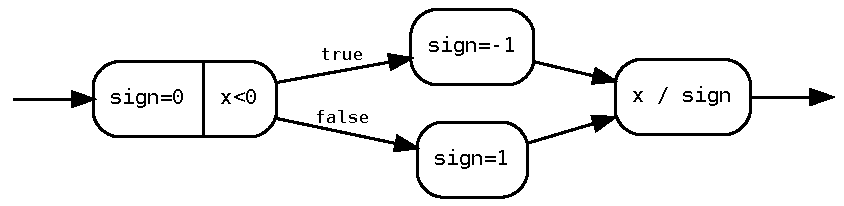
\includegraphics{Graphs/Examples_ifExampleCFG.pdf}
				\caption{The Control Flow Graph for the \code{ifExample} Method}
				\label{figure:positivecfg}
			\end{figure}

			\begin{figure}
				\centering
				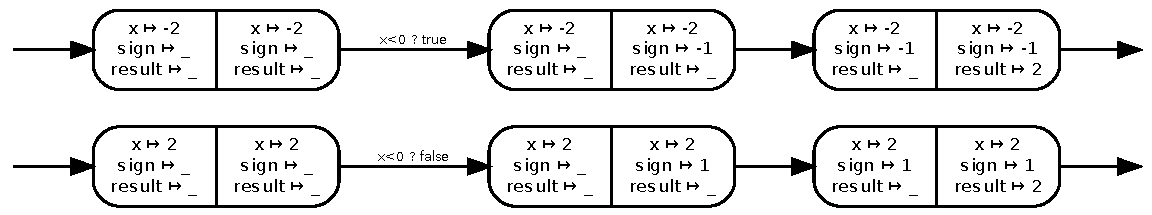
\includegraphics[width=\textwidth]{Graphs/Examples_ifExampleTransitionSystem.pdf}
				\caption{The Transition System}
				\label{figure:positivetransitionsystem}
			\end{figure}
		\end{example}

		There are several possible ways to define the semantics \concrete{P} of the program $P$. A hierarchical view of several possible definitions is given in \cite{cousot02}. The two relevant definitions for this presentation are the trace semantics and the collecting semantics.

		\begin{definition}[Trace]
			\label{definition:trace}
			A trace is a finite sequence of states $\sigma = \langle \sigma_0, \sigma_1, ..., \sigma_n \rangle$. The set of possible traces over the states $\Sigma$ is denoted by $\Sigma^\star$.
		\end{definition}

		With the definition of traces it is straightforward to define the first type of semantics, namely the trace semantics of a program $P$.

		\begin{definition}[Finite Partial Trace Semantics]
			\label{definition:tracesemantics}
			The finite partial trace semantics describes the set of traces that are determined by the transition system $P$.
			\begin{equation}
				\concrete{P} = \{\langle \sigma_0, \sigma_1, ..., \sigma_n \rangle \in \Sigma^\star \ | \ \sigma_0 \in \Sigma_0 \land \forall i, \sigma_i \to \sigma_{i+1} \}.
				\label{eq:tracesemantics}
			\end{equation}
		\end{definition}

		\begin{definition}[Trace Semantics as Fixed Point]
			\label{definition:TraceSemanticsFixedPoint}
			Alternatively, the trace semantics can be defined recursively as the least fixed point\footnote{The notion $\textbf{lfp}_{S_0}^{\subseteq} F$ represents the recursive application of $F$ starting with $S_0$ until $S_i = S_{i+1}$.}
			\begin{equation}
				\concrete{P} = \textbf{lfp}_{\Sigma_0}^{\subseteq}F_T
			\end{equation}
			of the semantic function $F_T$ defined as
			\begin{align}
				F_T: \Sigma^\star &\to \Sigma^\star\\
				S &\to S \cup \{ \langle \sigma_0, ..., \sigma_n, \sigma_{n+1} \rangle \ | \ \langle \sigma_0, ..., \sigma_n \rangle \in S \land \sigma_n \to \sigma_{n+1} \}. \notag
			\end{align}
		\end{definition}

		At each step of the iteration, all current traces in \concrete{P} are extended by all possible next states as defined by the transition relation. The resulting traces are then added to the set of current traces and the iteration starts over again. Starting with the set $\Sigma_0$ of initial states, this will enumerate all possible traces described by $P$. Note that \concrete{P} is not necessarily finite and the existence of a fixed point can therefore not be guaranteed.

		Given equation \ref{eq:tracesemantics}, we can define the semantics collecting the set of all reachable states as follows.

		\begin{definition}[Collecting Semantics]
			\label{definition:collectingsemantics}
			The states that are reachable in a given transition system are called collecting semantics
			\begin{equation}
				\collecting{P} = \{\sigma_n \ | \ \langle \sigma_0, ..., \sigma_n \rangle \in \concrete{P} \}.
			\end{equation}
		\end{definition}

		\begin{definition}[Collecting Semantics as Fixed Point]
			\label{definition:CollectingSemanticsFixedPoint}
			Analogously to the trace semantics, the collecting semantics can be written in fixed point form
			\begin{equation}
				\collecting{P} = \textbf{lfp}_{\Sigma_0}^{\subseteq}F_C
			\end{equation}
			using the semantic function $F_C$ defined as
			\begin{align}
				F_C: \Sigma &\to \Sigma\\
				S &\to S \cup \{ \sigma_{n+1} \ | \ \sigma_n \in S \land \sigma_n \to \sigma_{n+1} \}. \notag
			\end{align}
		\end{definition}

		The difference to the iteration computing the trace semantics is that, instead of keeping track of traces, the iteration only looks at single states. In every step, all next states of all current states, as described by the transition relation, are added to the set.

		\begin{example}[Semantics]
			The concepts presented so far can be illustrated looking at the transition system introduced by Figure \ref{figure:positivetransitionsystem}. Each trace of the system starts with an initial state from $\Sigma_0$. The two possible initial states are the states on the left side of the figure. The trace semantics contains all possible traces described by the system. To compute the trace semantics as a fixed point, we start with the two traces containing only the initial states. For each trace we then recursively add all possible nodes that are connected to the last state of a trace in the current set of traces. For this example this is a trivial task but note that this is merely due to the restrictive choice of $\Sigma_0$. Computing the collecting semantics is trivial as well, since all depicted states are obviously reachable from an initial state, they are all part of \collecting{P}. The fixed point computation follows along the same lines as the computation of the trace semantics.
		
			Note that in the general case, the semantics might not be computable. The set of initial states might be infinite, considering all possible values of \code{x}. Or it might be prohibitively large, for example, when looking at all possible 32-bit integers for \code{x}. 

			\exampleend
		\end{example}


		Since \collecting{P} in general is undecidable, it is very common to compute an over-approximation of this set and check whether some safety property holds in all states. This is already a form of abstraction, a concept which will be formalized in the next section.
	\end{section}

	% ABSTRACTION

	\begin{section}{Abstraction}
		\label{section:abstraction}
		A single state $\sigma \in \Sigma$ in the mathematical model might be as simple as containing just  a mapping from variables to values or it might be as complicated as the actual state of some hardware component. Whichever way, its complexity might be hindering in both formulating as well as verifying interesting properties. 

		Abstraction removes complexity by focusing on the important aspects of system. This results in two problem domains. The concrete domain of the mathematical structure in question and its simplification, called the abstract domain. Abstract interpretation addresses the problem of relating these two domains in a sound way. That is, how is it possible to guarantee that statements made about an abstract state allow sound conclusions about its concrete counterpart?

		% Lattices

		\begin{subsection}{Lattices}
			A part of the solution is provided by the restrictions put on the domains. It is necessary that these are complete lattices.
			
			\begin{definition}[Lattice] 
				\label{definition:lattice}
				A partially ordered set $(S, \sqsubseteq)$ is a lattice if for any two elements $s_0, s_1 \in S$
				\begin{itemize}
					\item there exists a unique \emph{least upper bound} $s_u \in S$ such that $s_0 \sqsubseteq s_u \land s_1 \sqsubseteq s_u$ denoted by $s_0 \sqcup s_1$,
					\item there exists a unique \emph{greatest lower bound} $s_l \in S$ such that $s_l \sqsubseteq s_0 \land s_l \sqsubseteq s_1$ denoted by $s_0 \sqcap s_1$.
				\end{itemize}
				A lattice is said to be complete if both the least upper bound and the greatest lower bound are defined for any subset of $S$. 
			\end{definition}
				
			Definition \ref{definition:lattice} implies that there exists a single element that is the lower bound of all other elements in $S$ called bottom and denoted by $\bot$. Correspondingly, the single element that is the upper bound of all other elements is called top and denoted by $\top$.

			\begin{example}[Complete Lattice]
				A typical example of complete lattices are type hierarchies like the one depicted in Figure \ref{figure:typelattice}. It shows a system with four types A, B, C and D where both C and D are subtypes of B. The top and bottom elements have their counterparts in most modern languages. In \scala, for example, the top element of the type hierarchy is represented by \code{Any} and the bottom element by the type \code{Nothing}. The ordering relation then corresponds to the ``subtype'', the least upper bound to the ``least common supertype'' and the greatest lower bound to the ``greatest common subtype'' relationships.
				\exampleend

				\begin{figure}
					\centering
					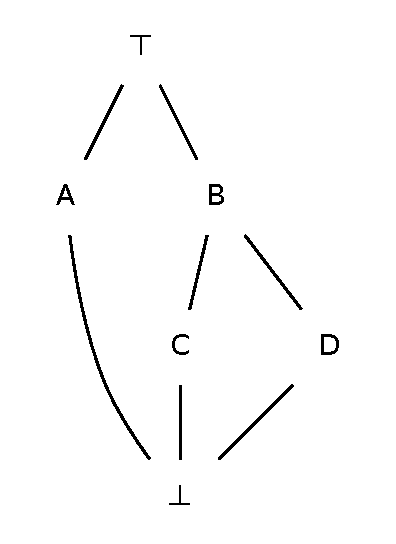
\includegraphics[scale=0.8]{Graphs/TypeLattice.pdf}
					\caption{A Type Lattice}
					\label{figure:typelattice}
				\end{figure}
			\end{example}

			To get an intuition about the function of these lattices it helps to think of their elements in terms of the information they represent. Taking the least upper bound of two elements corresponds to finding the minimum element that encompasses the information of both its arguments and results in a loss of precision. Taking the greatest lower bound means looking for the element representing the information both elements have in common. The top element then represents the information stored in all elements of the lattice together without discerning between single possibilities, which in effect amounts to knowing nothing. On the other end of the lattice, the bottom element represents the conjunction of all elements and, assuming we discern between more than a single state, amounts to a contradiction.
		\end{subsection}

		% Galois Connection

		\begin{subsection}{Galois Connections}
			Knowing the structure of the two domains, it is time to look at functions connecting a concrete domain $\Sigma$ and its associated abstract domain $D$. The abstraction maps concrete elements to their abstract counterparts and is usually denoted by $\alpha: \Sigma \to D$. The function mapping abstract elements to the concrete states they describe is called concretization and, by convention, is denoted by $\gamma: D \to \Sigma$.
			
			\begin{definition}[Galois Connection]
				\label{definition:GaloisConnection}
				The relation of the two domains is a sound abstraction if these two functions form a Galois connection $(\Sigma, \subseteq) \galois{\alpha}{\gamma} (D, \sqsubseteq)$ , that is:
				\begin{enumerate}
					\item $\alpha$ and $\gamma$ are monotone: $\forall \sigma, \ \sigma' \in \Sigma, \ \sigma \subseteq \sigma' \implies \alpha(\sigma) \sqsubseteq \alpha(\sigma')$ and vice versa.
					\item $\alpha \circ \gamma$ is reductive: $\forall d \in D, \ \alpha \circ \gamma(d) \sqsubseteq d$. 
					\item $\gamma \circ \alpha$ is extensive: $\forall \sigma \in \Sigma, \ \sigma \subseteq \gamma \circ \alpha(\sigma)$.
				\end{enumerate}
			\end{definition}

 			Once more, it helps to think in terms of information to develop the intuition about this formalization of sound abstractions. The first point ensures that a less precise element in the concrete domain results in a less precise abstraction and conversely a loss in precision in the abstract leads to a loss of precision in the concrete domain. The last two points are closely related and formalize that while the abstract counterpart of some element may describe more than just the original element, the converse relation does not hold for abstract elements. That is, by means of concretization and subsequent abstraction it is not possible to gain information in the abstract domain.

			\begin{example}[Galois Connection]
				To further illustrate the points just made, consider the concrete domain of a program describing a set of variables and the abstract domain provided by the type system depicted in Figure \ref{figure:typelattice} from the previous example. The monotonicity of abstraction ensures that given two variables \code{x} of type \code{C} and \code{y} of type \code{D}, the abstraction of their combination given by type \code{B} must be a supertype of \code{C} and \code{D}. Assuming that \code{x} and \code{y} are the only variables in the system, monotonicity on the concretization ensures that all variables of type \code{C} (that is \code{x}) are a subset of all variables of type \code{B} (\code{x} and \code{y}).

				To illustrate the necessity of a reductive $\alpha \circ \gamma$, assume that this restriction is violated. Then starting with \code{x}, applying the abstraction to get type \code{C} and continuing with the concretization of \code{C} would somehow result in a set that does not include \code{x}. This clearly does not represent the common intuition of a sound abstraction. Arguing for the necessity of the third property can be done along the same lines.
				\exampleend
			\end{example}
		\end{subsection}

		% Soundness of the Abstraction

		\begin{subsection}{Soundness of the Semantics}
			Since the full transition system of a program is usually not tractable, having related the static aspects of the system, it remains unclear what happens during the transitions of the system. Assuming that transitions in the concrete system follow a set of rules, corresponding rules for transitions in the abstract domain need to be defined. How these are defined depends on the abstract properties of interest. However, the abstract transitions need to fulfill certain restrictions in order to guarantee soundness.

			\begin{definition}[Soundness of Abstract Operations]
				\label{definition:soundnessofabstractoperations}
				Given a concrete transition rule $\ldbrack s \rdbrack_\Sigma: \wp(\Sigma) \to \wp(\Sigma)$ corresponding to a programs transition system, its abstract counterpart $\ldbrack s \rdbrack_D: D \to D$ preserves soundness if
				\begin{equation}
					\forall \sigma \in \wp(\Sigma), \ \alpha(\ldbrack s \rdbrack_\Sigma(\sigma)) \sqsubseteq \ldbrack s \rdbrack_D(\alpha(\sigma)).
				\end{equation}
			\end{definition}

			Executing an abstract operation in the abstract domain results in a new state which describes at least the states that resulted from the execution of the corresponding concrete operation in the concrete domain.
		\end{subsection}
	\end{section}

	\begin{section}{Static Analysis}
		\label{section:StaticAnalysis}
		Static analysis with abstract interpretation is based on the fixed point computation of the collecting semantics (cf. Definition \ref{definition:CollectingSemanticsFixedPoint}). However, instead of actually computing the semantics which might not be decidable, the iteration happens in the abstract domain. Starting with the abstract states representing the initial states of the concrete transition system, each transition of the concrete system is simulated with abstract operations until the set of abstract reachable states converges.

		This leads to two problems. First of all, what guarantees that a fixed point computed in the concrete domain corresponds to the fixed point computed in the abstract domain? This question is answered by the so called fixed point transfer theorem as described in \cite{mauborgne:rival05}.

		\begin{theorem}[Fixed Point Transfer]
			\label{theorem:FixedPointTransfer}
			Given two functions $F_\Sigma: \Sigma \to \Sigma$ and $F_D: D \to D$ then
			\begin{equation}
				\forall \sigma \in \Sigma, \ d \in D, \ \sigma \subseteq \gamma(d) \land F_\Sigma \circ \gamma \subseteq \gamma \circ F_D \implies \textbf{lfp}_\sigma^\subseteq F_\Sigma \subseteq \textbf{lfp}_d^\subseteq F_D
			\end{equation}
		\end{theorem}

		The premises for this theorem have already been established with the definition of the Galois connection.

		The second problem is that of convergence. It is obvious that for some programs, the domain could be of infinite height and hence the fixed point computation may not converge. This problem is addressed using the widening operator instead of the least upper bound, defined as follows:

		\begin{definition}[Widening]
			\label{definition:widening}
			The widening is a binary operator $\nabla$ in $D$ satisfying
			\begin{enumerate}
				\item $\forall d, d' \in D, d \sqsubseteq d \ \nabla \ d' \land d' \sqsubseteq d \ \nabla \ d'$
				\item For any sequence $(d_n)_{n \in \mathbb{N}}$, the recursive application of the widening operator to the elements of the sequence starting with some $d_0 \in D$ will eventually converge.
			\end{enumerate}
		\end{definition}

		Replacing the union used in the fixed point iteration with an operator satisfying the above definition ensures convergence. The widening operator is specific to the abstract domain.

		\begin{example}[Static Analysis]
			The following example will show a step by step static analysis using the principles presented so far. The basis for this example is again the method \code{ifExample}, shown in Listing \ref{listing:positivesource}, but this time with no restrictions on the initial memory state, that is $\Sigma_0 = \{l_0\} \times M$ where $l_0$ denotes the first program location. 
			
			The abstract domain of interest is the sign domain depicted in Figure \ref{figure:signlattice} that tracks whether a variable is positive, negative or zero. I will not formally define the abstract operations here, they, however, follow common sense. For example, a negative number multiplied by a negative number results in a positive number. The addition of a negative and a positive number could result in either one and the analysis therefore concludes the result to be $\top$.

			Figure \ref{figure:staticanalysis} outlines some of the basic stages of the analysis. \one shows the initial state before the first block as well as its successor state, added by a single iteration of $F_R$. The initial state is set to $\top$, meaning that nothing about the environment is assumed. After simulating the execution of the first block using the abstract operations, sign is guaranteed to be \code{0}, therefore its sign must also be \code{0}.
			
			\two shows a few steps further in the analysis where the two branch states are already added to the set of known reachable states. A notable difference between the two branches is that when taking the \code{false} branch, \cx could either be \code{0} or \code{+} and it must therefore be set to $\top$.

			\three shows the final state of the analysis. The initial state of the last block must combine the results of the two branches by computing the widening. This has the unfortunate consequence that the resulting state is pretty useless since the little knowledge gained about the sign variable during the computation of the branch is lost.

			Convergence is reached in a single iteration over the transition system since the sign domain is really simple and the program does not contain any loops. 
			\exampleend

			\begin{figure}
				\centering
				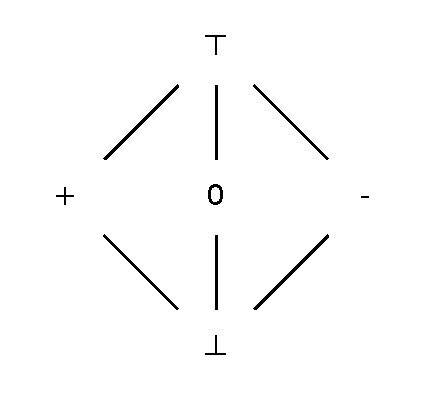
\includegraphics[scale=0.8]{Graphs/SignLattice.pdf}
				\caption{The Sign Lattice}
				\label{figure:signlattice}
			\end{figure}

			\begin{figure}[t]
				\centering
				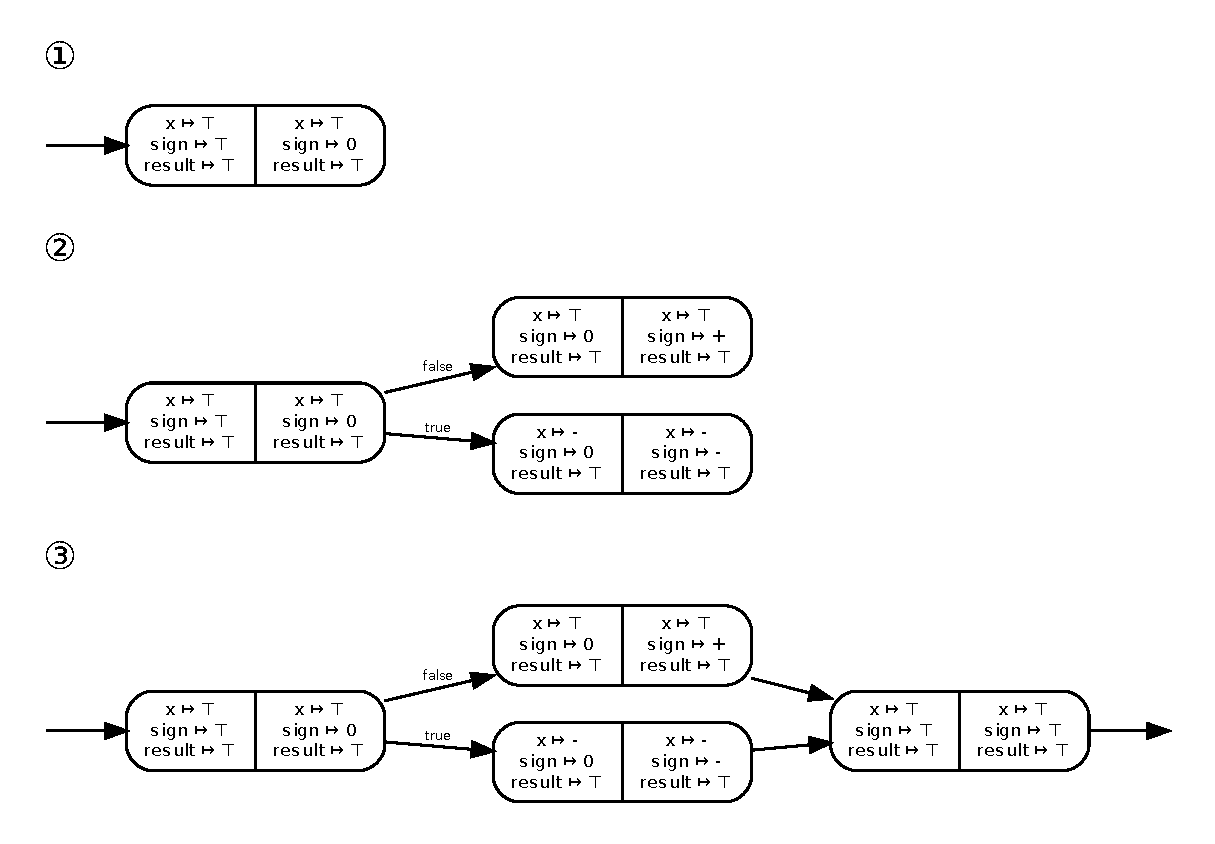
\includegraphics[width=\textwidth]{Graphs/StaticAnalysis.pdf}
				\caption{Step by Step Static Analysis}
				\label{figure:staticanalysis}
			\end{figure}
		\end{example}

	\end{section}

	\begin{section}{Example Domains}
		Having already hinted at the versatility of the abstract interpretation framework I am now going to provide a quick overview of some of the more commonly used abstract domains.

		\begin{subsection}{Numerical Domains}
			There are tons of domains addressing numerical issues. Although probably not that useful, but often used as an introductory example, the already presented sign domain is one of them. Another, more useful numerical domain is the interval domain which represents the value of a variable by a lower and an upper bound.

			The domains seen so far all represent values of single variables and are called non-relational domains. In contrast, relational domains try to, as their name already suggests, connect different variables. The prime example of this type of domain are the polyhedra described in \cite{cousot78}. They infer linear dependences between variables. The Octagons are another example of numerical domains. They track invariants of the from $\pm x \pm y \leq c$ and can be implemented efficiently as described in \cite{mine06}.
		\end{subsection}

		\begin{subsection}{Programming Language Features}
			The applicability of abstract interpretation is not limited to numerical domains. For example, most modern object oriented languages use some kind of a heap structure where objects reside in memory. Abstract interpretation can be used to argue about that structure, answering, for example, questions about aliasing.

			Furthermore, there are plenty of concepts that can be represented using an abstract domain lattice. To list just a few:
			\begin{itemize}
				\item The type system, using a lattice like the one depicted in Figure \ref{figure:typelattice}.
				\item Array indices, to prove the safety of array access operations.
				\item Information about string values \cite{costantini:ferrara:cortesi11}.
				\item Exhaustiveness of pattern matching for functional languages \cite{ferrara10}.
			\end{itemize}
		\end{subsection}

		These are just a few of the many possible domains, a search on Google-Scholar for ``abstract domain'' provides plenty of reading material for the interested reader.
	\end{section}
\end{chapter}

